\documentclass[11pt,a4paper]{article}

\usepackage[utf8]{inputenc}
\usepackage[T1]{fontenc}
\usepackage{lmodern}
\usepackage[english]{babel}
\usepackage{geometry}
\usepackage{graphicx}
\usepackage{float}
\usepackage{caption}
\usepackage{amsmath}
\usepackage{booktabs}
\usepackage{hyperref}
\usepackage{subcaption}
\usepackage{xcolor}

\geometry{margin=1in}
\raggedbottom

% Placeholder box for figures that will be added once the running jobs finish.
\newcommand{\figplaceholder}[1]{%
  \fbox{\parbox[c][4.2cm][c]{0.9\textwidth}{\centering\itshape
  \textcolor{gray}{[Figure to be inserted once the definitive runs finish: #1]}}}}

\title{Empirical Analysis of Transformers on Graph Connectivity \\
       \large Part III: Structural OOD Probes and a Faithful Paper Reproduction}
\author{Edoardo Paccagnella}
\date{\today}

\begin{document}

\maketitle

\section{Introduction}
\label{sec:intro}

This is the third report in the series. Parts~I and~II studied a
\emph{standard} (non-disentangled) transformer trained to predict the
connectivity matrix of an input graph, and asked whether the \emph{data
lever} of Ye, Fu, Jia and Sharan (2026) --- restricting the training data to
within-capacity graphs (diameter $\le 3^L$) --- helps a standard transformer
generalise out of distribution. The conclusion of Part~II was that, in our
$n = 40$ setup, the data lever speeds up convergence but does not produce the
predicted OOD benefit.

This report collects a new round of experiments. The first three sections are
targeted probes of \emph{what} the trained $n = 40$ models actually compute,
suggested as follow-ups to Part~II:
\begin{enumerate}
    \item \textbf{Cycle graphs (Section~\ref{sec:cycles}).} We test the four
          diameter-controlled $n = 40$ models on single cycles ($C_{40}$) and
          on pairs of disjoint cycles ($2 \times C_{20}$), two distributions
          that isolate the difference between confirming a long-range
          \emph{connection} and detecting a \emph{disconnection}.
    \item \textbf{Where the 2-chain error lives (Section~\ref{sec:pairwise}).}
          On 2-chains the models reach $\sim 80\%$ pairwise accuracy but
          $0\%$ exact match. We decompose the pairwise error to localise it.
    \item \textbf{Counting components (Section~\ref{sec:count}).} We train a
          new graph-level classifier to decide whether a graph is one chain
          or two chains (one vs.\ two connected components).
\end{enumerate}
The last section (Section~\ref{sec:repro}) reproduces the paper's
\emph{standard-transformer} preliminary experiment at $n = 20$. We report the
first test (the failure-to-generalise of Figure~1) and then explain why we are
re-running it with an architecture that matches the paper more faithfully
(three small RoBERTa-specific details), leaving space for the definitive
figures.

\section{Model and task}
\label{sec:model}

The task is unchanged from Parts~I--II. Given an undirected graph on $n$ nodes,
the input is its self-loop-augmented adjacency matrix
$A \in \{0,1\}^{n \times n}$ and the target is the connectivity matrix
$R \in \{0,1\}^{n \times n}$ with $R_{ij} = 1$ iff $i$ and $j$ lie in the same
connected component. We report \textbf{exact-match accuracy} (fraction of test
graphs predicted perfectly) and \textbf{pairwise accuracy} (fraction of
correctly predicted node pairs), optionally broken down by shortest-path
distance $d$.

Two model families appear in this report.

\paragraph{Large $n = 40$ connectivity models} (Sections~\ref{sec:cycles},
\ref{sec:pairwise}, \ref{sec:count}). These are exactly the large-model runs of
Part~II: $L = 2$ layers, $4$ attention heads, $d_{\mathrm{model}} = 512$,
$d_{\mathrm{ff}} = 2048$, normalised-ReLU attention
($\alpha = \tfrac{1}{n}\mathrm{ReLU}(QK^\top/\sqrt{d_h})$), pre-norm
LayerNorm, GELU feed-forward, no causal mask and no positional encoding;
$\sim 6.3$M parameters. They are trained on \textbf{Erd\H{o}s--R\'enyi
$\mathrm{ER}(n = 40, p = 0.05)$} graphs streamed online (each graph seen once,
$\approx 10^9$ graphs), batch size $1{,}000$, $1{,}000{,}000$ steps, AdamW with
peak learning rate $10^{-4}$, weight decay $10^{-4}$, cosine schedule, bf16.
The four runs differ only in the diameter filter applied to the training
stream: \emph{unfiltered}, $D \le 11$, $D \le 9$ ($= 3^L$), $D \le 7$.

\paragraph{Component classifier} (Section~\ref{sec:count}). Same trunk as
above, with the $n \times n$ read-out replaced by a mean-pool over node
embeddings followed by a single-logit head; trained with binary cross-entropy.

The reproduction of Section~\ref{sec:repro} uses a separate $n = 20$
configuration described in that section.

\section{Cycle graphs: connection vs.\ disconnection}
\label{sec:cycles}

\subsection{Setup}

\paragraph{Models.} The four large $n = 40$ connectivity models of
Section~\ref{sec:model}, trained on $\mathrm{ER}(n = 40, p = 0.05)$
(unfiltered, $D \le 11$, $D \le 9$, $D \le 7$).

\paragraph{Test distributions.} Two structured families, both on the full
$n = 40$ nodes (no isolated padding; $n_{\text{active}} = 40$), each a test set
of $10{,}000$ graphs with random node permutations:
\begin{itemize}
    \item \textbf{1cycle:} a single cycle $C_{40}$ through all $40$ nodes ---
          one connected component, every node of degree $2$, diameter $20$.
          The target $R$ is the all-ones matrix.
    \item \textbf{2cycle:} two disjoint cycles $2 \times C_{20}$ --- two
          connected components of $20$ nodes each, every node of degree $2$,
          component diameter $10$. The target $R$ is block-diagonal.
\end{itemize}
These two distributions are extreme opposites: on 1cycle a model must confirm
that \emph{every} pair is connected (including pairs at distance up to $20$),
whereas on 2cycle it must additionally \emph{cut} the graph into the two
correct components.

\subsection{Results}

\begin{table}[H]
\centering
\begin{tabular}{lcccc}
\toprule
 & \multicolumn{2}{c}{1cycle ($C_{40}$)} & \multicolumn{2}{c}{2cycle ($2\times C_{20}$)} \\
\cmidrule(lr){2-3}\cmidrule(lr){4-5}
Model & Exact match & Pairwise & Exact match & Pairwise \\
\midrule
Unfiltered & 0.000 & 0.748 & 0.000 & 0.729 \\
$D \le 11$ & \textbf{0.943} & \textbf{1.000} & 0.000 & 0.500 \\
$D \le 9$  & 0.000 & 0.475 & 0.000 & \textbf{0.975} \\
$D \le 7$  & 0.000 & 0.360 & 0.000 & 0.860 \\
\bottomrule
\end{tabular}
\caption{Exact-match and pairwise accuracy of the four $n = 40$ models on the
two cycle test sets ($10{,}000$ graphs each, $n_{\text{active}} = 40$). Bold
marks the best model in each column.}
\label{tab:cycles}
\end{table}

\begin{figure}[H]
    \centering
    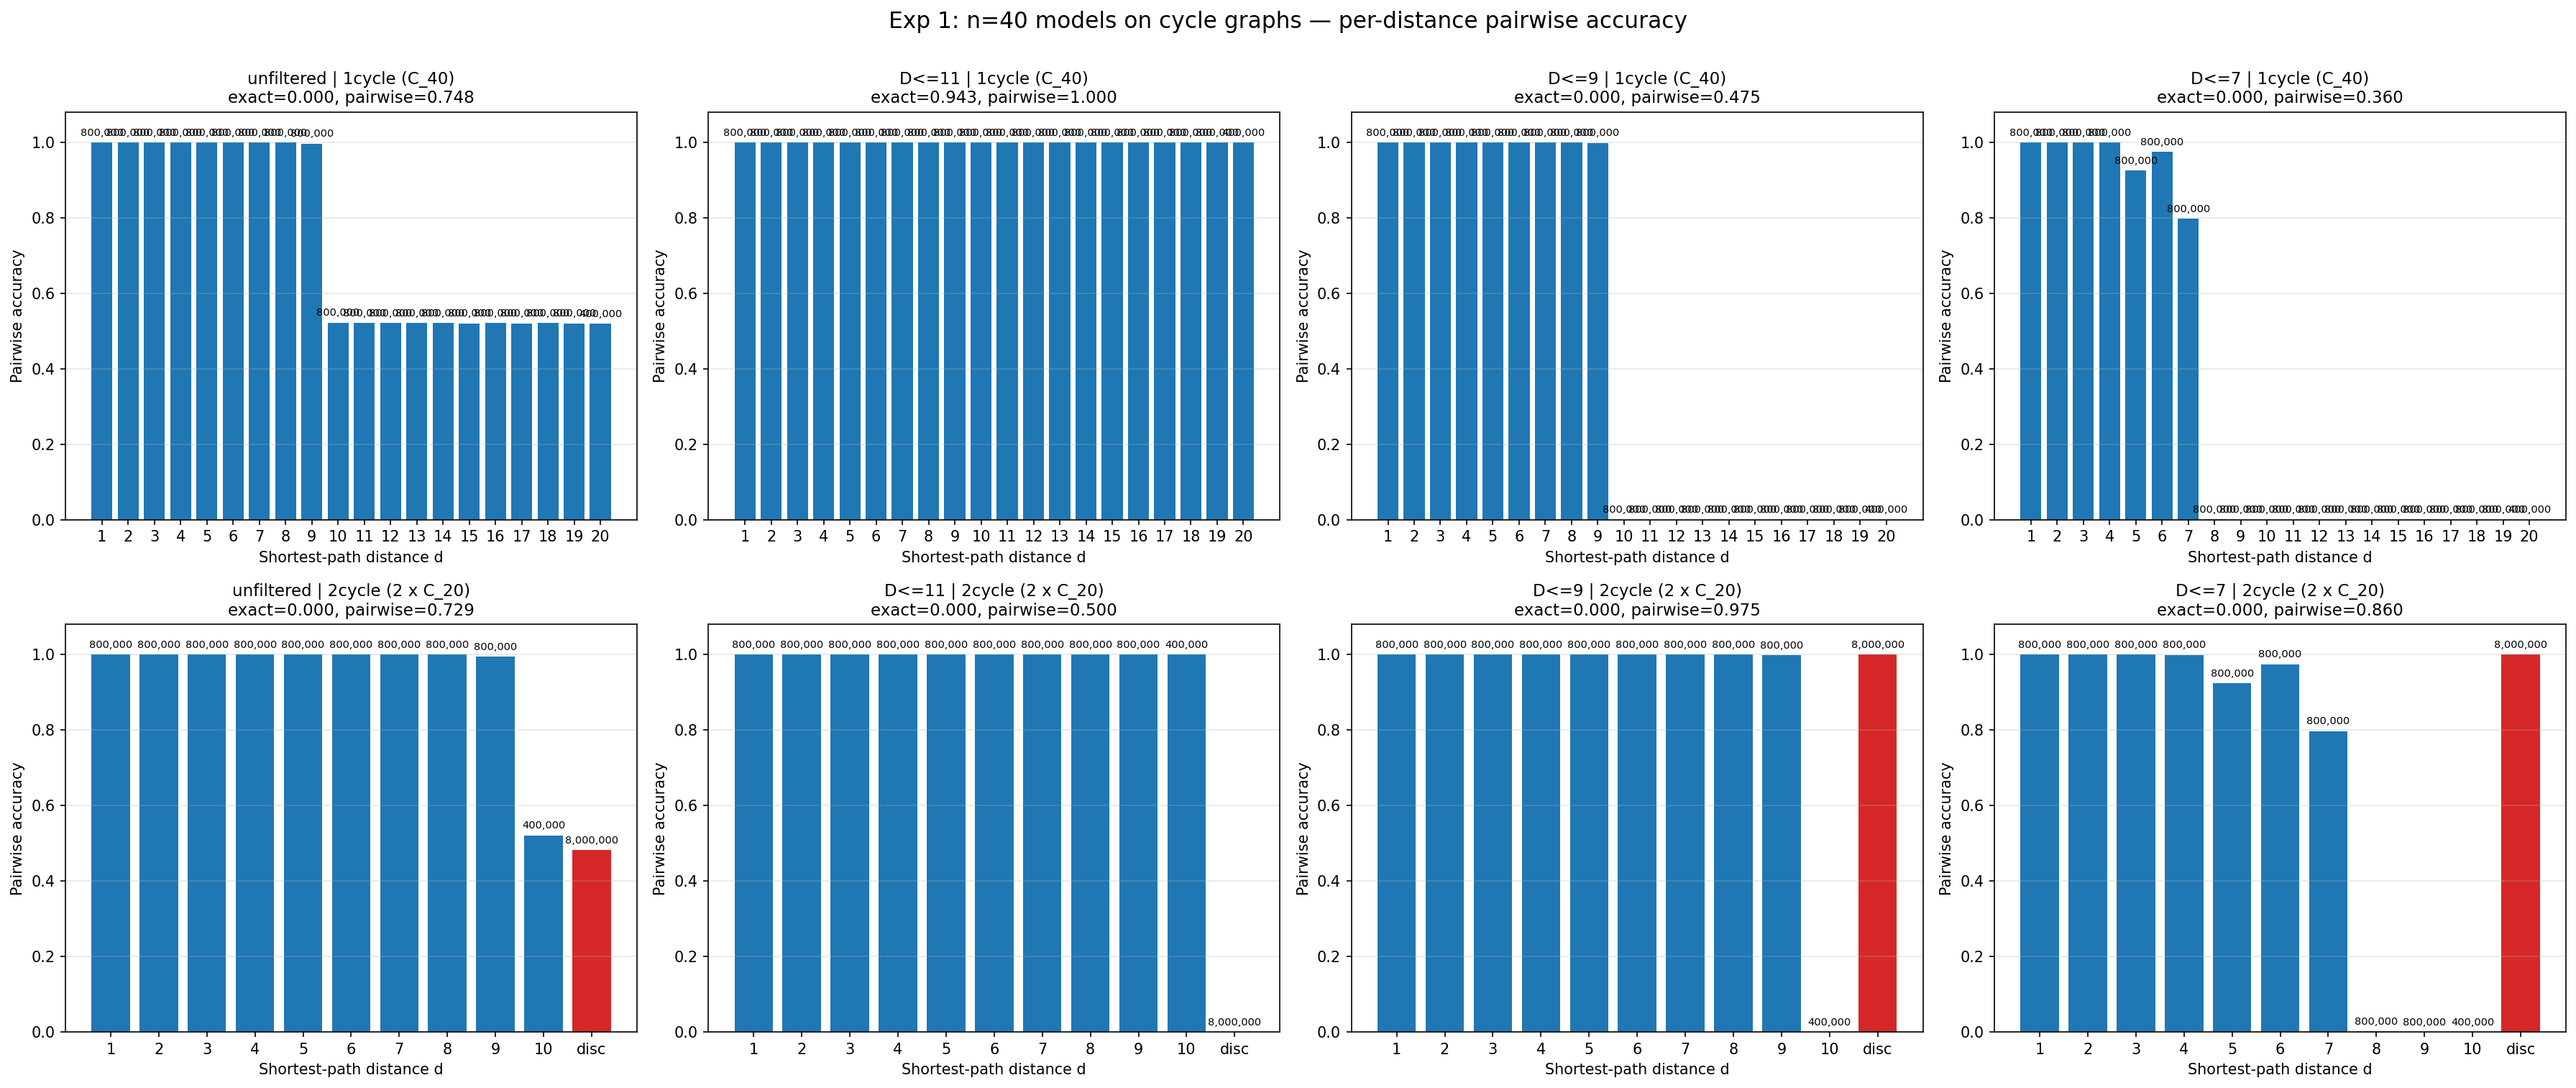
\includegraphics[width=\textwidth]{runs/n40_cross_experiment/cycles_per_distance_big.png}
    \caption{Per-distance pairwise accuracy on the cycle test sets. Rows:
    1cycle (top) and 2cycle (bottom); columns: the four diameter-controlled
    models. The number above each bar is the count of test pairs at that
    distance; the red bar is the ``disconnected'' (across-component) bin.}
    \label{fig:cycles}
\end{figure}

\paragraph{What the table and figure show.} There is a clean cross-over.
The $D \le 11$ model is best on 1cycle (pairwise $1.000$, exact $0.943$) but
collapses to chance ($0.500$) on 2cycle: it behaves like ``predict connected
everywhere'', which is exactly right when the graph is a single component and
exactly $50\%$ wrong when it is two. The tightly filtered models $D \le 9$ and
$D \le 7$ are the mirror image: they are best at \emph{separating} the two
cycles ($0.975$ and $0.860$ on 2cycle) but poor on 1cycle ($0.475$, $0.360$),
because a single $C_{40}$ requires confirming connections up to distance $20$,
far beyond their effective range. The unfiltered model sits in between
($\approx 0.73$ on both). In short, a tighter diameter budget trades the
ability to confirm long-range connection for the ability to detect
disconnection --- the capacity trade-off the paper predicts.

\section{Where the 2-chain error lives}
\label{sec:pairwise}

\subsection{Setup}

\paragraph{Models.} The same four large $n = 40$ models trained on
$\mathrm{ER}(n = 40, p = 0.05)$.

\paragraph{Test distribution.} \textbf{2-chains} at the full size
$n = 40$, $k = n/2 = 20$: two disjoint paths of $20$ nodes each (two connected
components), random node permutations, $5{,}000$ graphs. This is the
$n_{\text{active}} = 40$ case requested as a follow-up to Part~II; note that a
$20$-node path has diameter $19$, so it contains within-component pairs at
distances well beyond the capacity $3^L = 9$.

On this distribution the models reach $\sim 80\%$ pairwise accuracy but $0\%$
exact match, and Part~II showed (Figure on 2-chains by $n_{\text{active}}$) the
exact-match accuracy collapses from $1.0$ to $0.0$ exactly at
$n_{\text{active}} = 22$. We decompose the pairwise error to understand the
$80\%$ figure. For each model we split the off-diagonal pairs into:
within-component pairs at distance $d \le 9$ (within capacity), within-component
pairs at $d > 9$ (beyond capacity), and across-component pairs (target $0$). As
a reference we also report the \emph{capacity oracle}, the predictor
``connected $\iff 1 \le d \le 9$''.

\subsection{Results}

\begin{table}[H]
\centering
\begin{tabular}{lcccccc}
\toprule
Model & Overall & \multicolumn{1}{c}{within $d\!\le\!9$} & within $d\!>\!9$ & across (disc.) & pred-conn.\ rate \\
\midrule
Unfiltered & 0.821 & 1.000 & 0.263 & 0.855 & 0.458 \\
$D \le 11$ & 0.825 & 0.993 & 0.221 & 0.879 & 0.437 \\
$D \le 9$  & \textbf{0.853} & 0.983 & 0.000 & \textbf{1.000} & 0.340 \\
$D \le 7$  & 0.788 & 0.794 & 0.000 & \textbf{1.000} & 0.275 \\
\midrule
Capacity oracle & 0.859 & 1.000 & 0.000 & 1.000 & --- \\
\bottomrule
\end{tabular}
\caption{Off-diagonal pairwise accuracy on 2-chains $(n = 40, k = 20)$, split
by target class and within-component distance. ``pred-conn.\ rate'' is the
fraction of off-diagonal pairs the model predicts as connected. The last row is
the capacity oracle ``connected $\iff d \le 9$''. Bold marks the best model per
column.}
\label{tab:pairwise}
\end{table}

\begin{figure}[H]
    \centering
    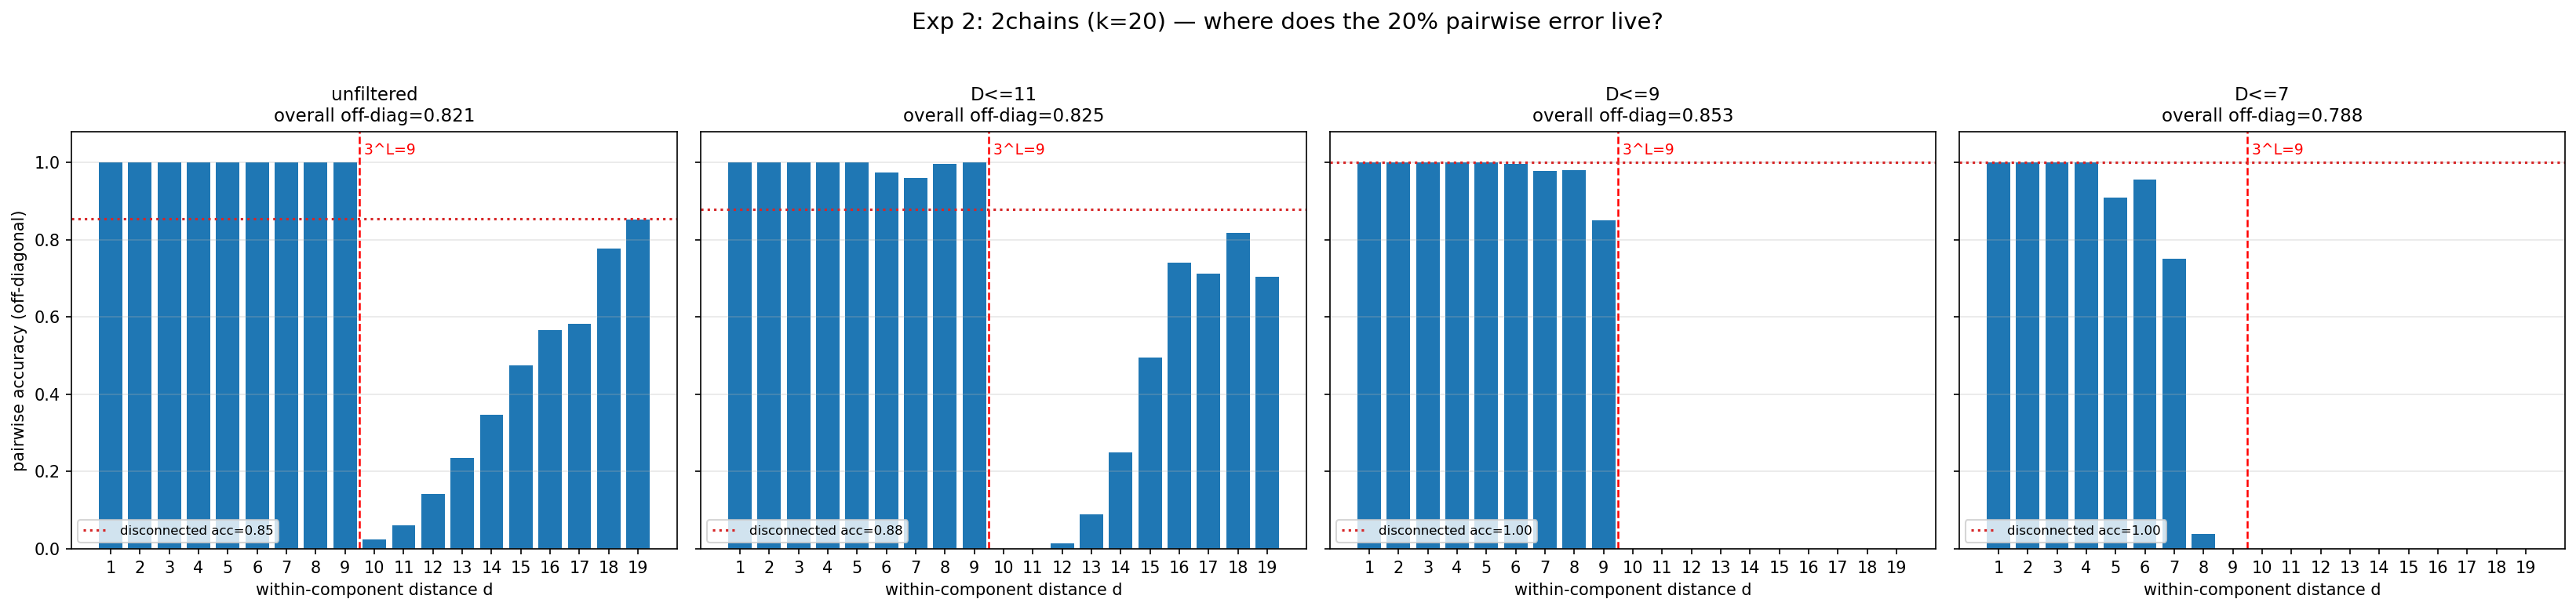
\includegraphics[width=\textwidth]{runs/n40_cross_experiment/diagnose_2chains_k20.png}
    \caption{Per-distance pairwise accuracy on 2-chains $(k = 20)$ for the four
    models. The dashed red line marks the capacity $3^L = 9$; the dotted red
    line is the across-component (disconnected) accuracy. Accuracy is near
    perfect up to $d = 9$ and collapses beyond it.}
    \label{fig:diagnose}
\end{figure}

\begin{figure}[H]
    \centering
    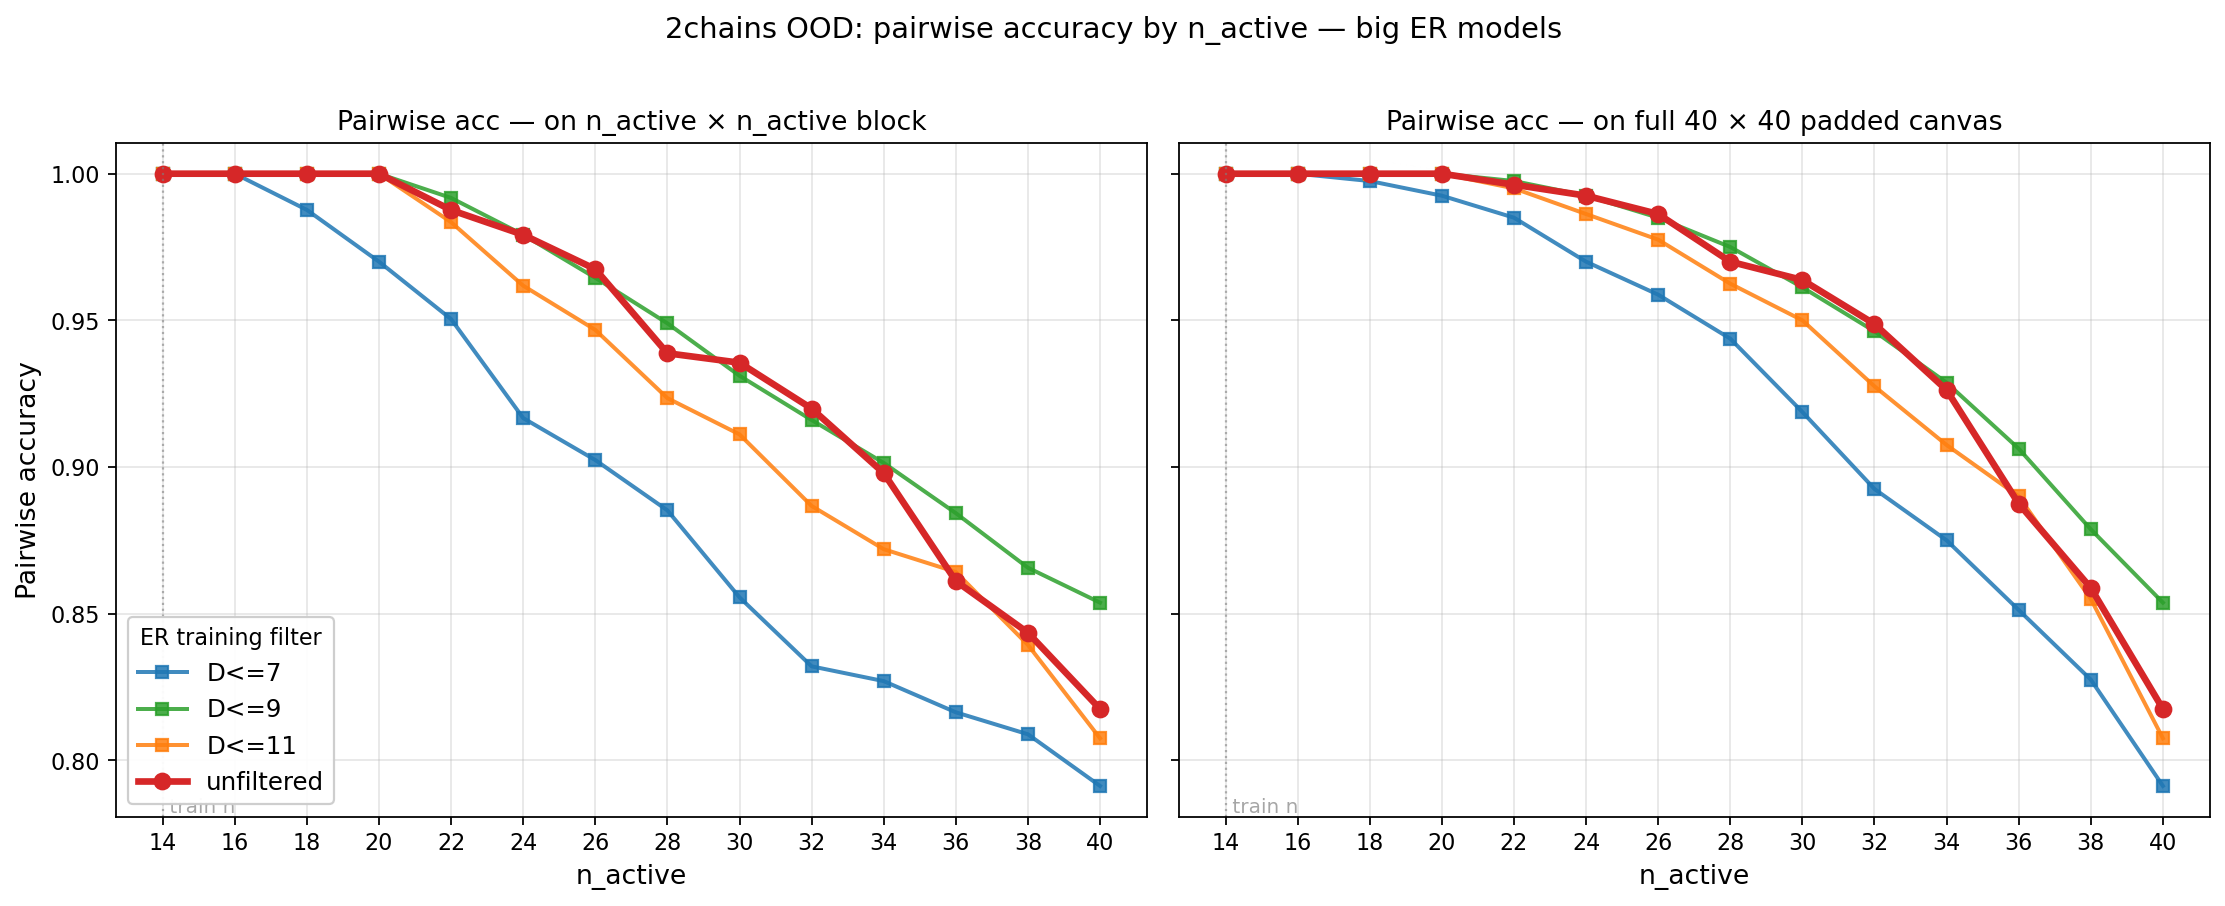
\includegraphics[width=0.9\textwidth]{runs/n40_cross_experiment/two_chains_pairwise_by_n_active_big.png}
    \caption{2-chains pairwise accuracy as a function of $n_{\text{active}}$
    (left: measured on the active $n_{\text{active}} \times n_{\text{active}}$
    block; right: on the full $40 \times 40$ canvas), for the four models. The
    accuracy stays high even where exact match is already $0$.}
    \label{fig:byn}
\end{figure}

\paragraph{What the table and figures show.} The $\sim 80\%$ pairwise accuracy
is not a heuristic artefact: the error is concentrated almost entirely in the
\emph{within-component pairs beyond capacity} ($d > 9$). The capacity-respecting
models $D \le 9$ and $D \le 7$ get every across-component pair right
(disconnected accuracy $1.000$, zero false positives) and every within-capacity
pair right, but score exactly $0.000$ on $d > 9$ pairs --- they implement
``connected $\iff d \le 9$''. Indeed the $D \le 9$ model ($0.853$) is within
$0.6$ points of the capacity oracle ($0.859$). Because every 2-chain with
$k = 20$ contains pairs at distances $10$--$19$, every graph has some wrong
pairs, which is why exact match is $0$ while pairwise stays high. This also
explains the cliff at $n_{\text{active}} = 22$ reported in Part~II:
$n_{\text{active}} = 20$ means chains of length $10$ (maximum distance $9 =$
capacity), the last fully solvable size; $n_{\text{active}} = 22$ introduces
distance $10 > 9$ and breaks exact match.

\section{Counting components: 1-chain vs.\ 2-chain}
\label{sec:count}

\subsection{Setup}

\paragraph{Task.} A new \emph{graph-level binary} task: decide whether the input
graph is a single chain (one connected component, label $0$) or two chains (two
connected components, label $1$). This is the ``$+1$ for 2-chains, $-1$ for
1-chain'' classification, mapped to BCE targets $\{1, 0\}$.

\paragraph{Architecture.} The component classifier of Section~\ref{sec:model}:
the same large $n = 40$ trunk ($d_{\mathrm{model}} = 512$, $4$ heads,
$d_{\mathrm{ff}} = 2048$, normalised-ReLU attention, $2$ layers) with a
mean-pool + single-logit head. AdamW, peak lr $10^{-4}$, weight decay
$10^{-4}$, cosine schedule, batch size $1{,}000$, $200{,}000$ steps, bf16.

\paragraph{Training and test distributions.} Online stream at $n = 40$, $50/50$
between a \textbf{1-chain} (a single path over all $40$ nodes) and a
\textbf{2-chain} ($k = 20$: two disjoint paths of $20$ nodes), node order
randomly permuted. The two classes are nearly indistinguishable by cheap global
cues: both use all $40$ nodes, the edge counts are $39$ vs.\ $38$, and the
degree histograms differ only by $2$ vs.\ $4$ degree-$1$ endpoints. The test set
is balanced ($5{,}000$ of each class). We ran \textbf{2 iterations}
(seeds $1000$, $2000$).

\subsection{Results}

\begin{table}[H]
\centering
\begin{tabular}{lcccc}
\toprule
Seed & Best accuracy & 1-chain acc.\ & 2-chain acc.\ & Step to acc.\ $\ge 0.99$ \\
\midrule
$1000$ & 1.000 & 1.000 & 1.000 & $2{,}000$ \\
$2000$ & 1.000 & 1.000 & 1.000 & $2{,}000$ \\
\bottomrule
\end{tabular}
\caption{1-chain vs.\ 2-chain classification at $n = 40$. Both seeds reach
$100\%$ balanced accuracy at the first evaluation ($2{,}000$ steps).}
\label{tab:count}
\end{table}

\begin{figure}[H]
    \centering
    \begin{subfigure}[t]{0.48\textwidth}
        \centering
        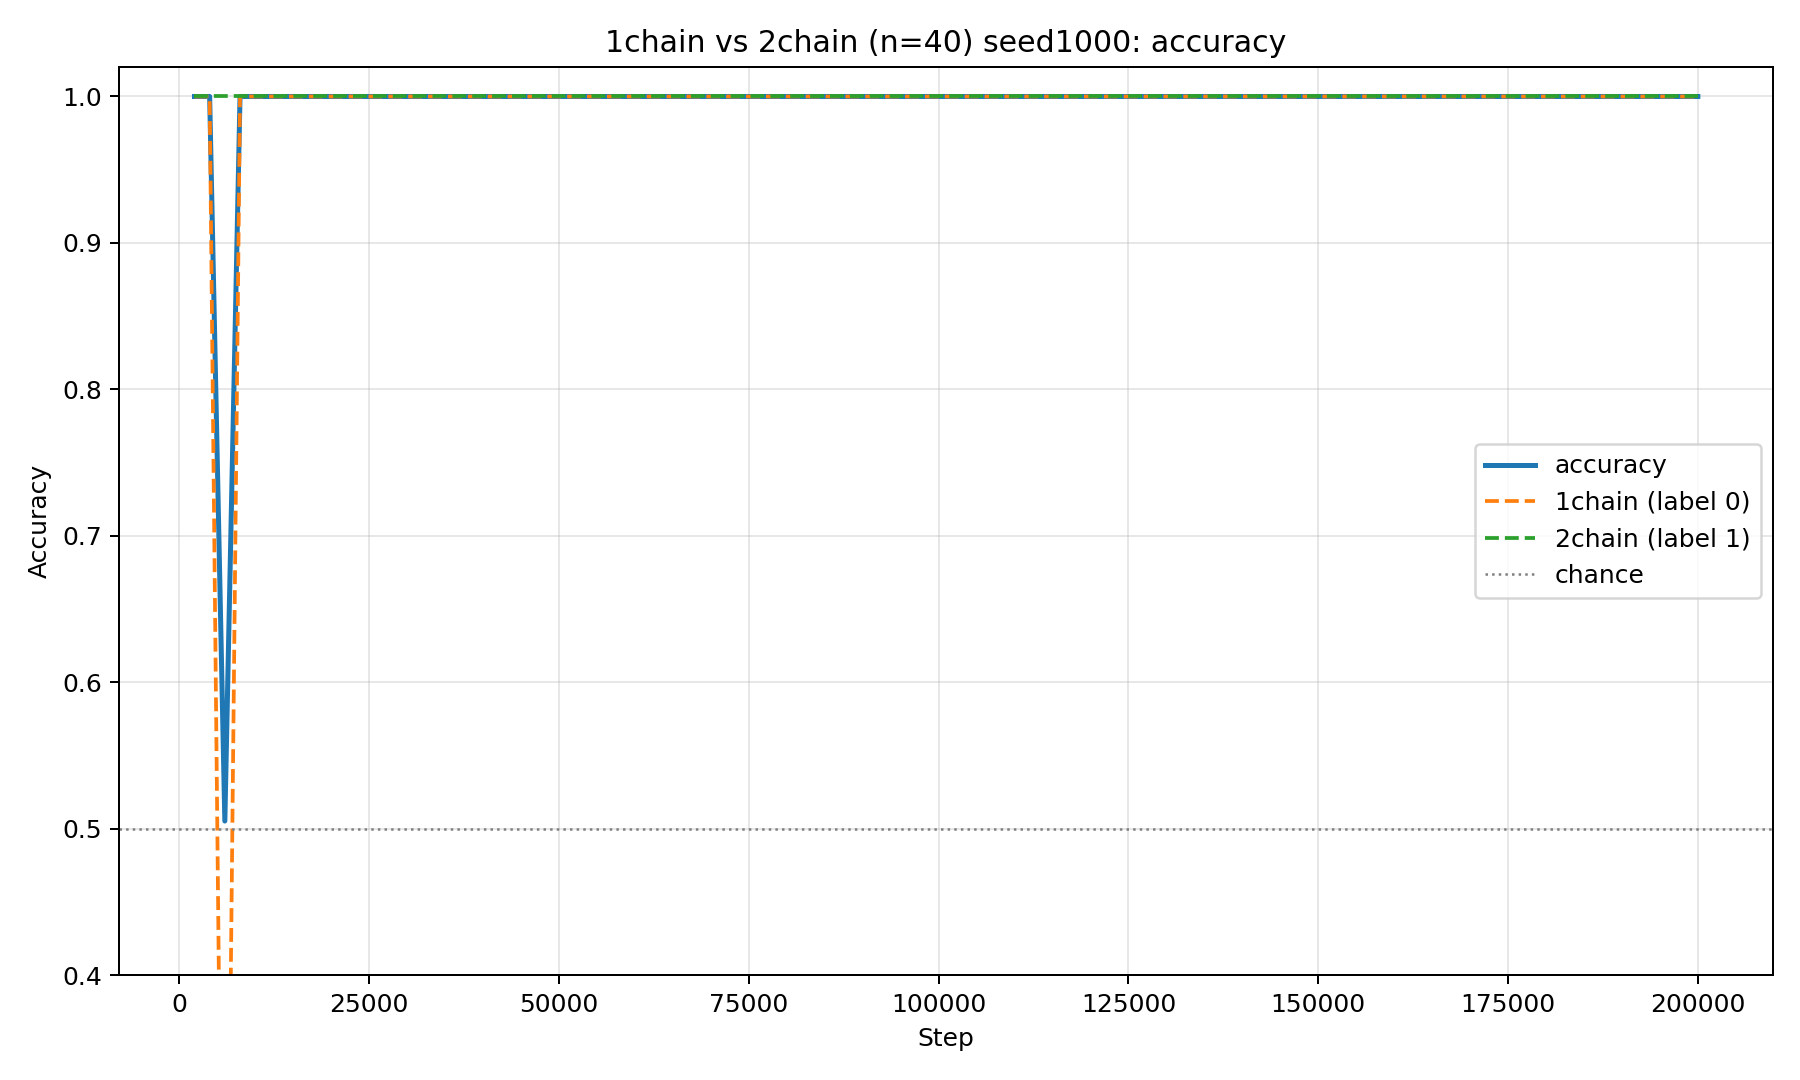
\includegraphics[width=\textwidth]{runs/exp3_chaincount/chaincount_n40_seed1000/chaincount_n40_seed1000_accuracy.png}
        \caption{Seed $1000$.}
    \end{subfigure}
    \hfill
    \begin{subfigure}[t]{0.48\textwidth}
        \centering
        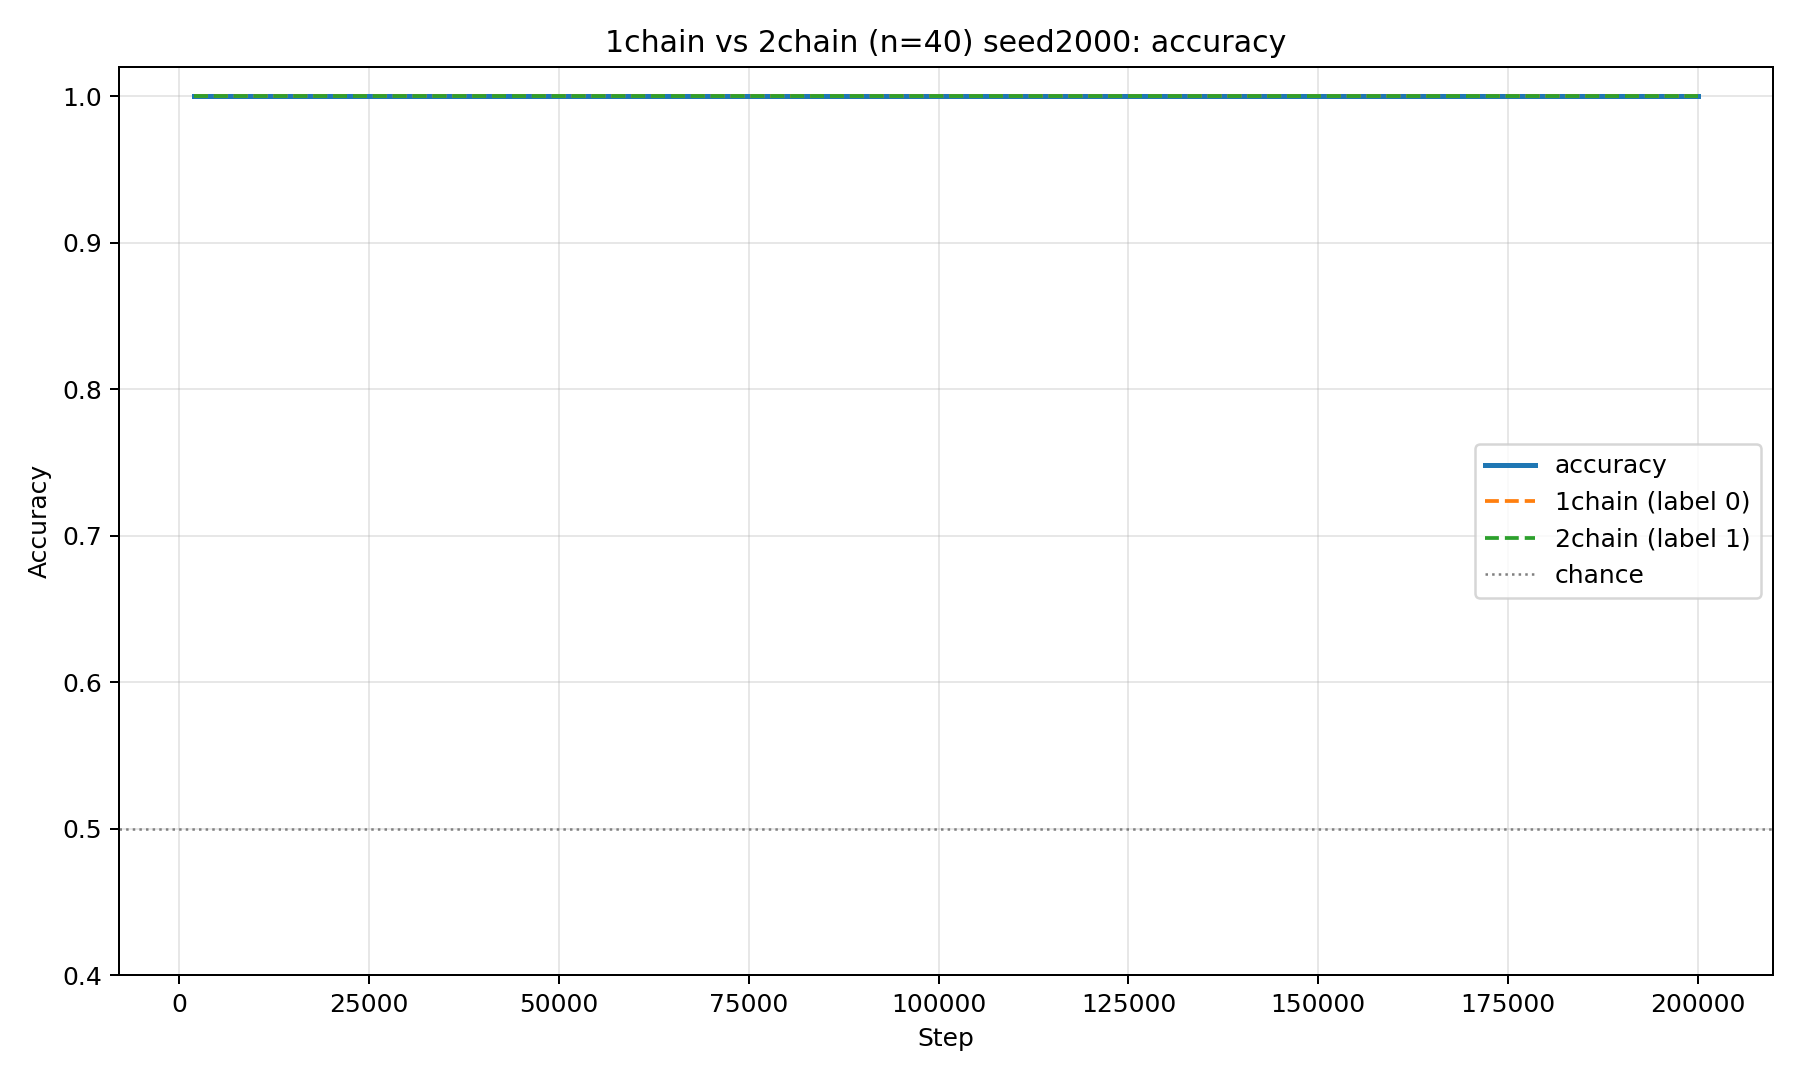
\includegraphics[width=\textwidth]{runs/exp3_chaincount/chaincount_n40_seed2000/chaincount_n40_seed2000_accuracy.png}
        \caption{Seed $2000$.}
    \end{subfigure}
    \caption{Balanced classification accuracy vs.\ training step for the two
    iterations (overall, and per class). The dashed line is chance ($0.5$).}
    \label{fig:count}
\end{figure}

\paragraph{What the table and figures show.} Counting components ($1$ vs.\ $2$)
is trivial for this architecture: both seeds reach $100\%$ accuracy within
$2{,}000$ steps. This is a sharp contrast with Section~\ref{sec:pairwise}: the
same trunk \emph{cannot} produce the full connectivity matrix of a 2-chain
(exact match $0$), yet it \emph{can} instantly report that the graph has two
components. The bottleneck of the connectivity task is therefore not sensing the
global structure but producing correct long-range, per-pair reachability ---
the $3^L$ wall --- not detecting disconnection per se.

\section{Reproducing the paper's standard-transformer experiment ($n = 20$)}
\label{sec:repro}

\subsection{Setup}

\paragraph{Goal.} Reproduce the paper's preliminary standard-transformer study
(its Figure~1, and the data-lever Figures~7 and~11) under \emph{exactly} the
paper's configuration, to compare directly with our $n = 40$ findings.

\paragraph{Architecture.} As specified in the paper (\S3.3 and Appendix~A.1/D.1):
a $2$-layer standard transformer, \textbf{single-head} self-attention,
$d_{\mathrm{model}} = 512$, $d_{\mathrm{ff}} = 2048$, normalised-ReLU attention
$\alpha = \tfrac{1}{n}\mathrm{ReLU}(QK^\top/\sqrt{d_h})$, pre-norm LayerNorm,
GELU feed-forward, no positional encoding. AdamW, peak lr $10^{-4}$, weight
decay $10^{-4}$, cosine schedule, batch size $1{,}000$, $1{,}000{,}000$ steps,
each graph seen once ($\approx 10^9$ graphs), bf16.

\paragraph{Training and test distributions.} Training on
\textbf{$\mathrm{ER}(n = 20, p = 0.08)$}, in two conditions: \emph{unrestricted}
and \emph{restricted} to diameter $\le 9$ ($= 3^L$, the data lever). Test on the
two out-of-distribution families used by the paper, both at $n = 20$:
\textbf{2Chain$(n = 20, k = 10)$} (two disjoint paths of $10$ nodes) and
\textbf{2Clique$(n = 20, k = 10)$} (two disjoint $10$-cliques). We ran
\textbf{3 iterations} (seeds $1000$, $2000$, $3000$) per condition. The metric
is exact-match accuracy, exactly as in the paper (\S3.3: the product over all
node pairs).

\subsection{First test: in-distribution success, OOD failure (Figure~1)}

\begin{table}[H]
\centering
\begin{tabular}{llccc}
\toprule
Condition & Seed & ER (in-dist) & 2Chain & 2Clique \\
\midrule
Unrestricted & $1000$ & 1.000 & 0.065 & 0.000 \\
Unrestricted & $2000$ & 1.000 & 0.046 & 0.000 \\
Unrestricted & $3000$ & 1.000 & 0.071 & 0.000 \\
\midrule
Restricted $D \le 9$ & $1000$ & 1.000 & 0.034 & 0.000 \\
Restricted $D \le 9$ & $2000$ & 1.000 & 0.017 & 0.000 \\
Restricted $D \le 9$ & $3000$ & 1.000 & 0.051 & 0.000 \\
\bottomrule
\end{tabular}
\caption{Reproduction with the minimal (clean A.1-style) architecture:
exact-match accuracy at the end of training. In distribution every run is
perfect; both OOD families stay near zero, \emph{including} the
diameter-restricted runs. (For reference, 2Chain pairwise accuracy is
$\approx 0.99$ and 2Clique pairwise $\approx 0.50$ across all runs.)}
\label{tab:repro-min}
\end{table}

\begin{figure}[H]
    \centering
    \begin{subfigure}[t]{0.48\textwidth}
        \centering
        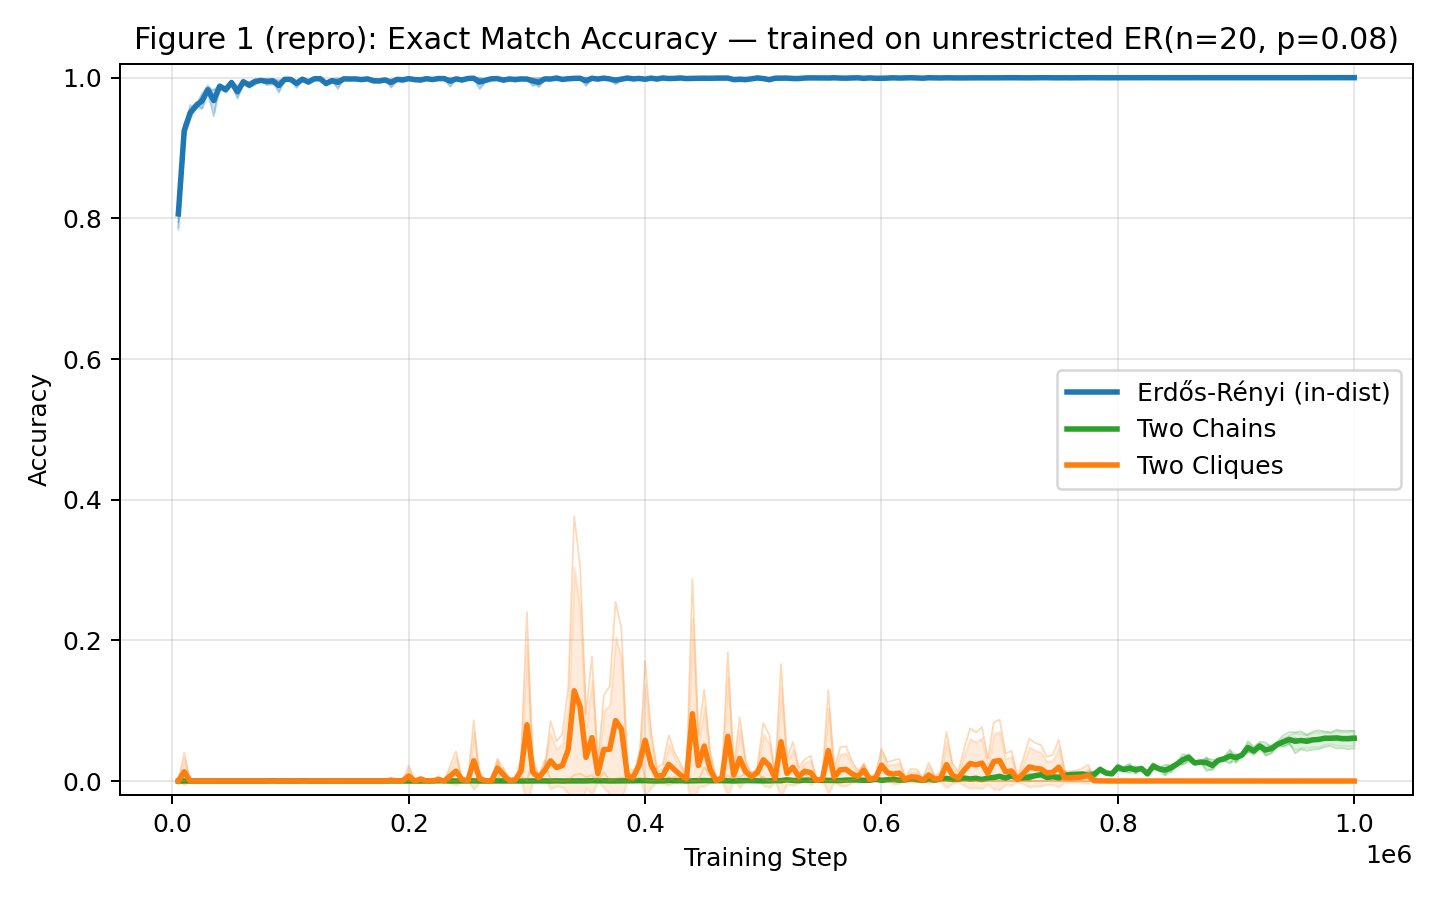
\includegraphics[width=\textwidth]{runs/repro_paper_n20/fig1_reproduction.png}
        \caption{Our reproduction (minimal architecture, mean over $3$ seeds):
        exact-match accuracy vs.\ training step for the unrestricted model on
        ER (in-distribution), 2Chain and 2Clique.}
    \end{subfigure}
    \hfill
    \begin{subfigure}[t]{0.48\textwidth}
        \centering
        \figplaceholder{RoBERTa-faithful Figure~1}
        \caption{RoBERTa-faithful architecture (definitive run, in progress).}
    \end{subfigure}
    \caption{Figure~1 reproduction. In distribution the model is perfect; the
    two OOD families stay near zero --- matching the paper's Figure~1, which
    shows that the standard transformer fails to generalise. The right panel
    is reserved for the definitive RoBERTa-faithful run.}
    \label{fig:repro-fig1}
\end{figure}

\paragraph{What the table and figure show.} The \emph{first} test reproduces the
paper cleanly: in distribution the model is perfect (ER exact $= 1.000$ for all
$3$ seeds), and on the OOD 2Chain/2Clique families exact match is essentially
zero. This is the failure-to-generalise of the paper's Figure~1. However, the
\emph{data lever} (the restricted $D \le 9$ rows) does \emph{not} reproduce the
paper's Figures~7/11 here: the restricted runs fail just like the unrestricted
ones, contrary to the paper, where restriction recovers $\sim 0.9$ on 2Chain.

\subsection{Why we re-ran it: a slightly different architecture}

Inspecting the paper carefully, we found that our reproduction above used a
clean ``Definition~A.1'' transformer, whereas the paper (Appendix~D.1) states it
\emph{``adopts the implementation from RoBERTa with single-head per layer and
normalised-ReLU attention''}. ``Adopting RoBERTa'' carries three engineering
details that our minimal model did not match:
\begin{enumerate}
    \item \textbf{post-LayerNorm} blocks (LayerNorm after the residual add), as
          in BERT/RoBERTa, instead of pre-LayerNorm;
    \item \textbf{dropout $0.1$} (RoBERTa default), instead of no dropout;
    \item \textbf{weight initialisation} $\mathcal{N}(0, 0.02)$ (RoBERTa
          default), instead of the framework default.
\end{enumerate}
(We also removed two unintended biases of the minimal model --- the output
symmetrisation and an extra final LayerNorm --- so that the read-out matches
A.1 exactly.) These details govern the training dynamics, and the paper's claim
is precisely about which solution gradient descent selects; they are therefore a
plausible reason the algorithmic phase transition appears for the paper and not
for our minimal model. We re-ran all $6$ experiments (the two conditions
$\times$ $3$ seeds) with this RoBERTa-faithful architecture, everything else
identical. The definitive figures are reported below once the runs finish.

\subsection{Definitive results: RoBERTa-faithful architecture}

\begin{figure}[H]
    \centering
    \figplaceholder{RoBERTa-faithful reproduction of Figure~1 (ER / 2Chain / 2Clique vs.\ step, mean over 3 seeds)}
    \caption{Figure~1, RoBERTa-faithful. (To be inserted:
    \texttt{runs/repro\_paper\_n20\_roberta/fig1\_reproduction.png}.)}
    \label{fig:repro-rob-fig1}
\end{figure}

\begin{figure}[H]
    \centering
    \figplaceholder{RoBERTa-faithful reproduction of Figure~7 (2Chain exact match: unrestricted vs.\ restricted $D\le9$)}
    \caption{Figure~7, RoBERTa-faithful: the data lever on 2Chain. (To be
    inserted: \texttt{runs/repro\_paper\_n20\_roberta/fig7\_reproduction.png}.)}
    \label{fig:repro-rob-fig7}
\end{figure}

\begin{figure}[H]
    \centering
    \figplaceholder{RoBERTa-faithful reproduction of Figure~11 (2Clique exact match: unrestricted vs.\ restricted $D\le9$)}
    \caption{Figure~11, RoBERTa-faithful: the data lever on 2Clique. (To be
    inserted: \texttt{runs/repro\_paper\_n20\_roberta/fig11\_reproduction.png}.)}
    \label{fig:repro-rob-fig11}
\end{figure}

\paragraph{Comment.} The question these definitive runs answer is whether the
three RoBERTa details are enough to make the data lever work: does the
restricted ($D \le 9$) model generalise to 2Chain/2Clique (the paper's
Figures~7/11) where the minimal model did not? Early signal from the
unrestricted runs already suggests the RoBERTa architecture can reach the
algorithmic solution (high seed variance), unlike the minimal model; the
restricted runs and the full $3$-seed comparison will be added here.

\end{document}
